
\section{Gantt Chart}

A Gantt chart was used to give myself a high-level overview of how my time should be spent so that I would have appropriate time to complete the necessary aspects of this project. This was useful in prioritising different aspects and knowing when to plan deadlines for myself (for example, having a hard cut-off point for my implementation).
\x
Figure~\ref{fig:gantt-chart-1} shows the Gantt chart for this project up util the progress report submission, which includes the planning and design phases.

\begin{figure}[H]
  \centering
  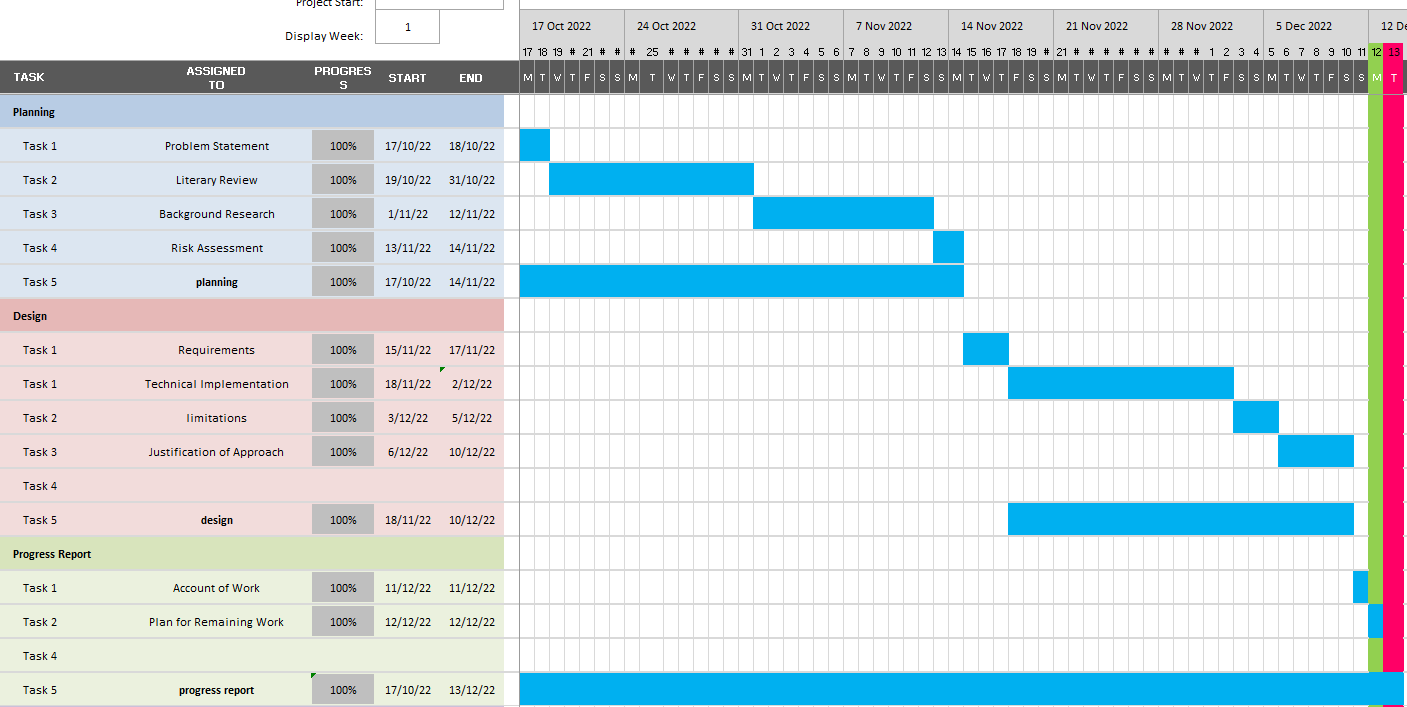
\includegraphics[width=\textwidth]{assets/images/charts/gantt/progress.png}
  \caption{Gantt Chart leading up to the progress report}
  \label{fig:gantt-chart-1}
\end{figure}

\noindent Figure~\ref{fig:gantt-chart-2} shows the Gantt chart for the implementation phase of this project. The implementation phase was split into three sprints, as detailed in Section~\ref{sec:sprints}, each with their own planning phase.

\begin{figure}[H]
  \centering
  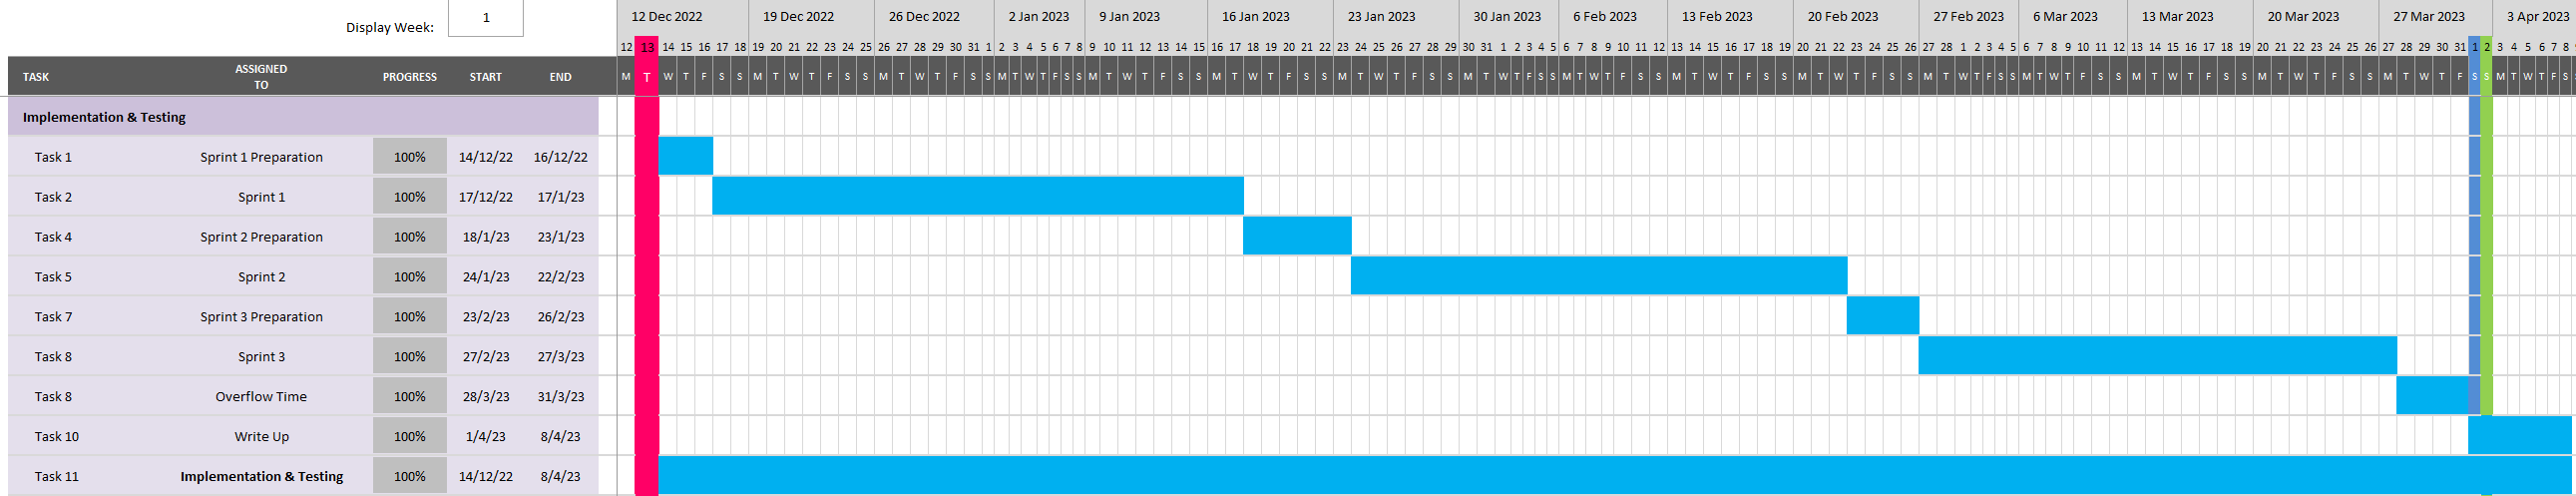
\includegraphics[width=\textwidth]{assets/images/charts/gantt/impl.png}
  \caption{Gantt Chart showing the three sprints}
  \label{fig:gantt-chart-2}
\end{figure}

\noindent Figure~\ref{fig:gantt-chart-3} shows the Gantt chart for the final testing and evaluation phases of my application. As I used test-driven development, the testing phase only needed to consist of acceptance and benchmark testing among some other fixes. 

\begin{figure}[H]
  \centering
  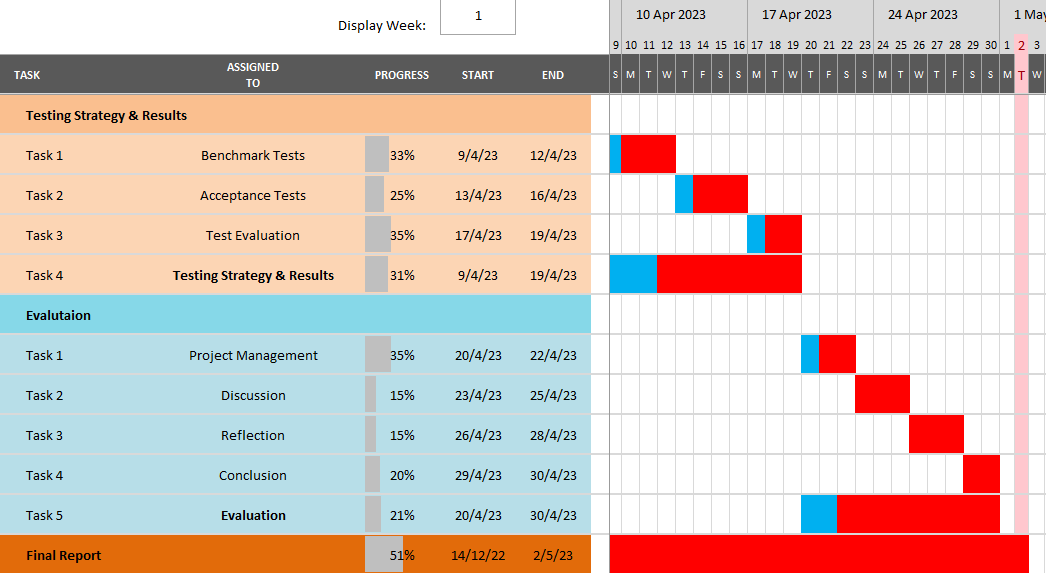
\includegraphics[width=\textwidth]{assets/images/charts/gantt/testing-eval.png}
  \caption{Gantt Chart showing the final testing and evaluation}
  \label{fig:gantt-chart-3}
\end{figure}